\begin{frame}{range min-Max tree (rmM-tree)}
    \begin{itemize}
        \item Árvore binária completa, baseada em intervalos de tamanho $b$;
        \item Cada nó cobre valores de excessos dentro de um intervalo;
        \item Construção bottom-up;
        \item Complexidade de espaço igual à $n + O(\frac{n}{b} \log n)$ bits;
        \item Operações realizadas em tempo $O(\log n)$.
    \end{itemize}
\end{frame}

\begin{frame}{range min-Max tree binária}
    \begin{figure}[h!]
        \centering
        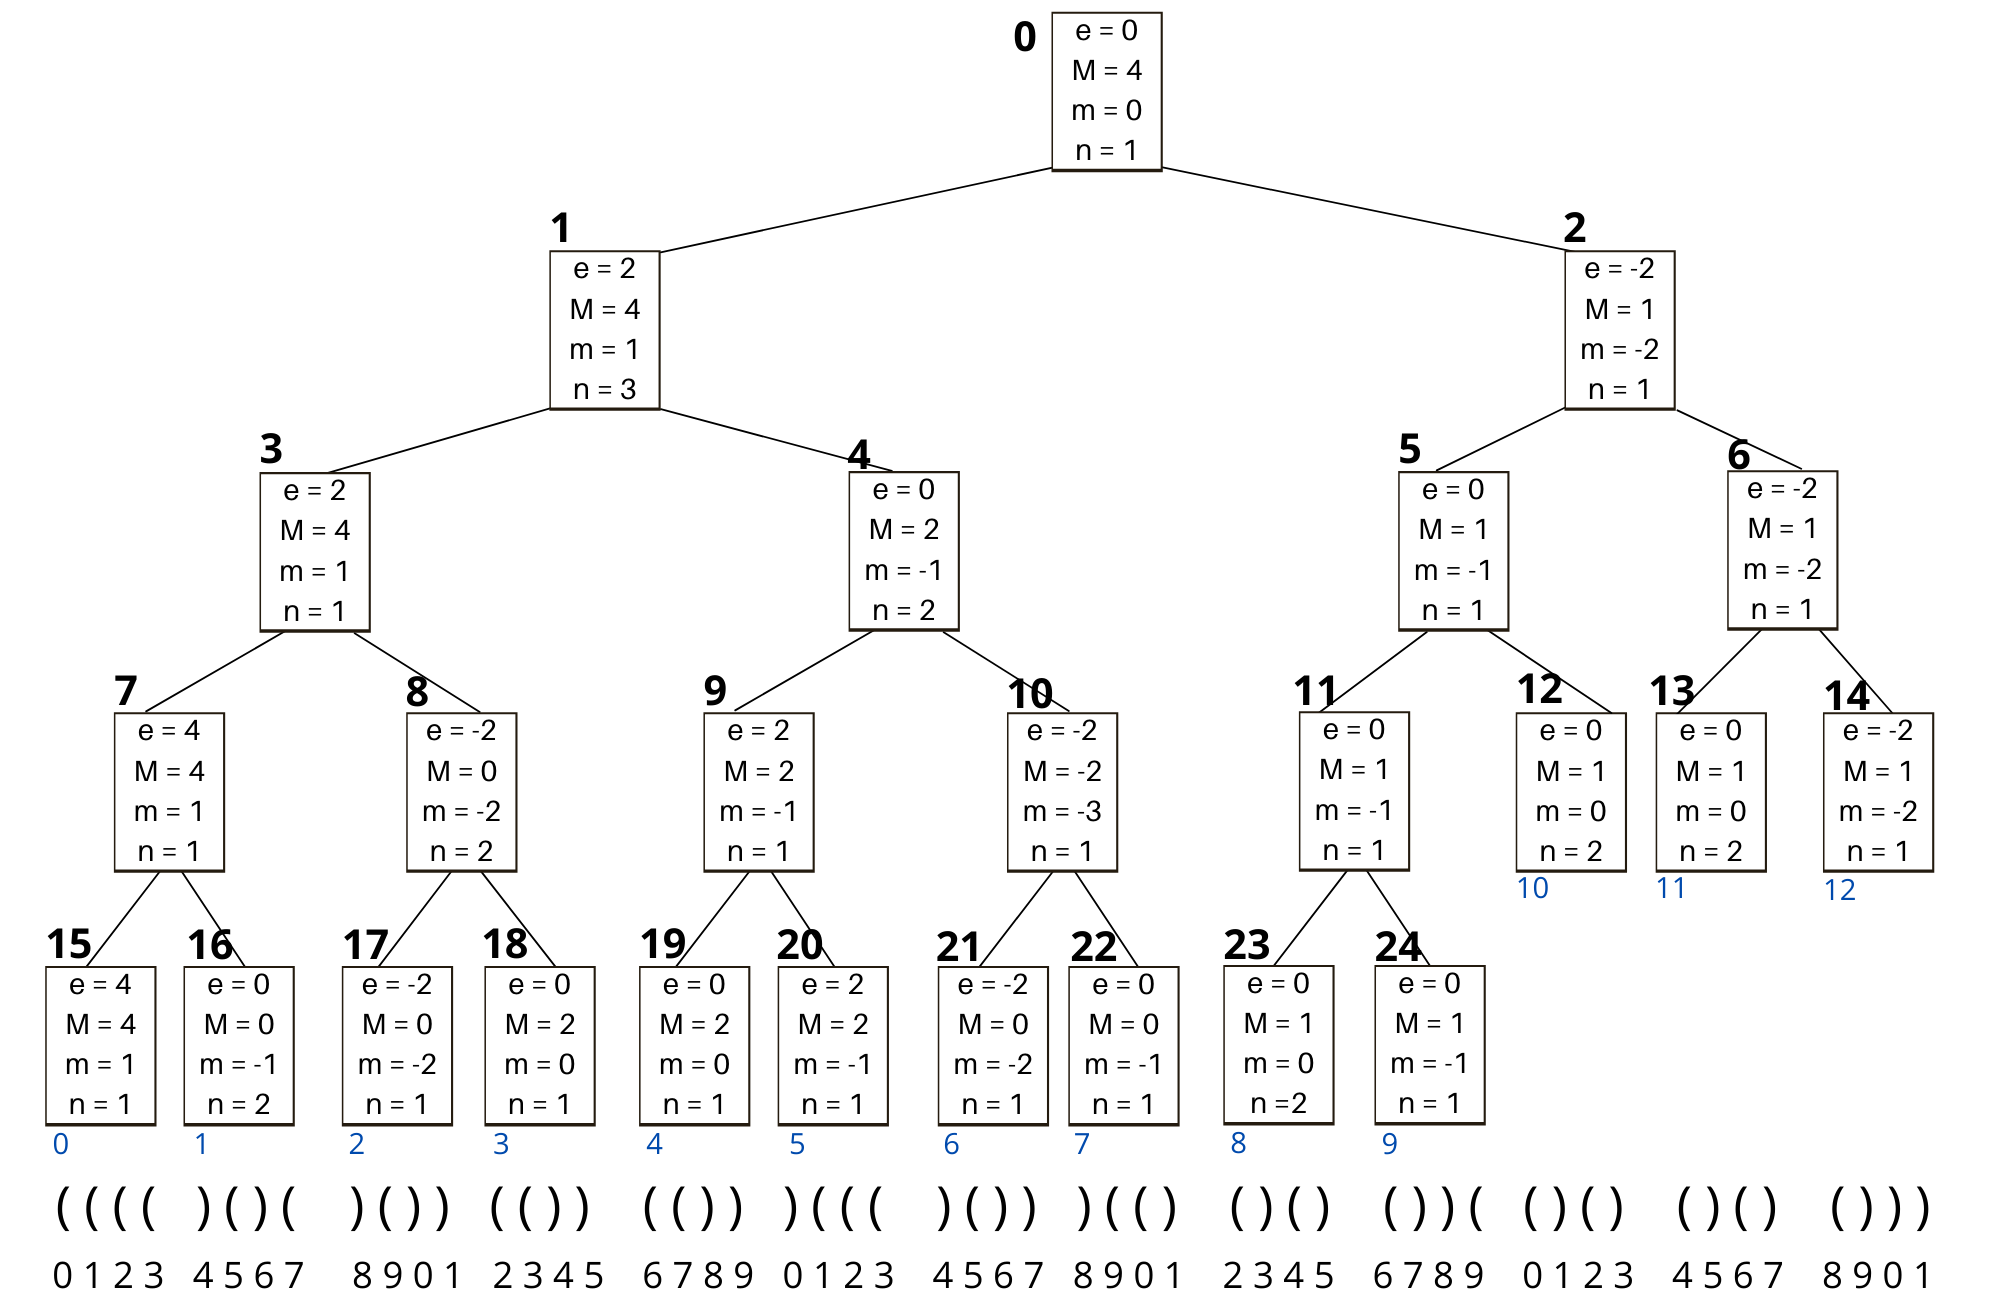
\includegraphics[scale=0.3]{images/rmm-tree-bin.png}\\
        \caption{rmM-tree binária com blocos de tamanho 4}
    \end{figure} 
\end{frame}

\begin{frame}{rmM-tree: Registros}

    \textbf{Valores de excesso}
        Dado um nó $v$ que cobre um intervalo $BP[s,e]$, então:
        \begin{itemize}
            \item $R[v].e$: excesso total no intervalo\\
            $R[v].e = excess(e)-excess(s-1)$.
            \item $R[v].M$: excesso máximo no intervalo\\
            $R[v].M = \max\{excess(i) - excess(s - 1) | s \leq i \leq e\}$.
            \item $R[v].m$: excesso mínimo no intervalo\\
            $R[v].m = \min\{excess(i) - excess(s - 1) | s \leq i \leq e\}$.
            \item $R[v].n$: número de vezes que o excesso mínimo ocorre no intervalo\\
            $R[v].n = |\{BP[i]=R[v].m | s \leq i \leq e\}|$.
        \end{itemize}
\end{frame}

\begin{frame}{rmM-tree: Registros}
    \textbf{Nós internos e raíz}
    \begin{figure}[h]
        \begin{minipage}[c]{0.35\linewidth}
            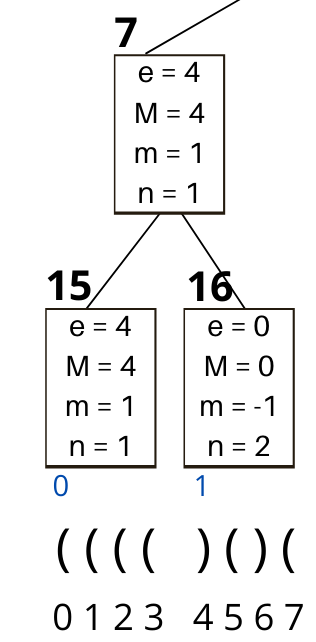
\includegraphics[scale=0.65]{images/internal-nodo.png}
        \end{minipage}
        \begin{minipage}[c]{0.49\linewidth}
            \begin{tabular}{l}\\
                R[7].e = R[15].e +  R[16].e.             \\
                R[7].M=max(R[15].M, R[15].e+ R[16].M).\\
                R[7].m=min(R[15].m, R[15].e+ R[16].m). \\
                R[7].n= R[15].n. \\
            \end{tabular}
        \end{minipage}
    \end{figure}
\end{frame}

\begin{frame}{rmM-tree: Operações}
    \begin{table}[]
       \begin{tabular}{|c|c|c|}
            \hline
            \multicolumn{3}{|c|}{\textbf{Operações}}  \\ \hline  
            fwdsearch(i,d)                       &bwdsearch(i,d)                        &minExcess(i,j) \\ \hline               
            maxExcess(i,j)                       & minSelectExcess(i,j,t)               & minCount(i,j)                       \\ \hline
            enclose(i)                           & rank\_v(i)                           & select\_v(i)                         \\ \hline                                
            findClose(i)                         & findOpen(i)                          & rmq(i,j) \\ \hline
            inspect(i)                           & preRank(i)                           & postRank(i)                    \\ \hline
            preSelect(i)                         & postSelect(i)                        & isLeaf(i)                       \\ \hline
            isAncestor(i,j)                      & depth(i)                             & parent(i)   \\ \hline
        \end{tabular}
    \end{table}
\end{frame}

\begin{frame}{rmM-tree: Operações}
    \begin{table}[]
        \begin{tabular}{|c|c|c|}
        \hline
        \multicolumn{3}{|c|}{\textbf{Operações}}                                                         \\ \hline
        firstChild(i) &  lastChild(i) & nextSibling(i) \\ \hline
        prevSibling(i)    & subtreeSize(i)                   & levelAncestor(i,d)         \\ \hline
        \multicolumn{1}{|c|}{level-next(i)} & levelPrev(i)  & \multicolumn{1}{c|}{levelLmost(d)} \\ \hline
        levelRmost(d)                      & lca(i,j)       & deepestNode(i)                     \\ \hline
        degree(i)                           & child(i,q)     & childRank(i)                       \\ \hline
        leafRank(i)                        & leafSelect(i) & lmostLeaf(i)                       \\ \hline
        \end{tabular}
    \end{table}
\end{frame}


\begin{frame}{rmM-tree: operações}
    Problema 1: Dado um nó codificado em $i=1$, encontrar o nó codificado em $j>i$, mais à esquerda de $i$.


    Solução: 
    $$nextSibling(i) = findClose(i) +1$$ 


    $$findClose(i) = fwdSearch(i,-1)$$ 
 \end{frame}

 \begin{frame}{rmM-tree: operações}
    $$fwdSearch(i,d) = min\{ j > i | excess(j) = excess(i) + d \}$$ 
 \end{frame}

 \begin{frame}{rmM-tree: $nextSibling$}
    Problema 1: Computar $nextSibling(1)$.
     \begin{figure}[h!]
         \centering
         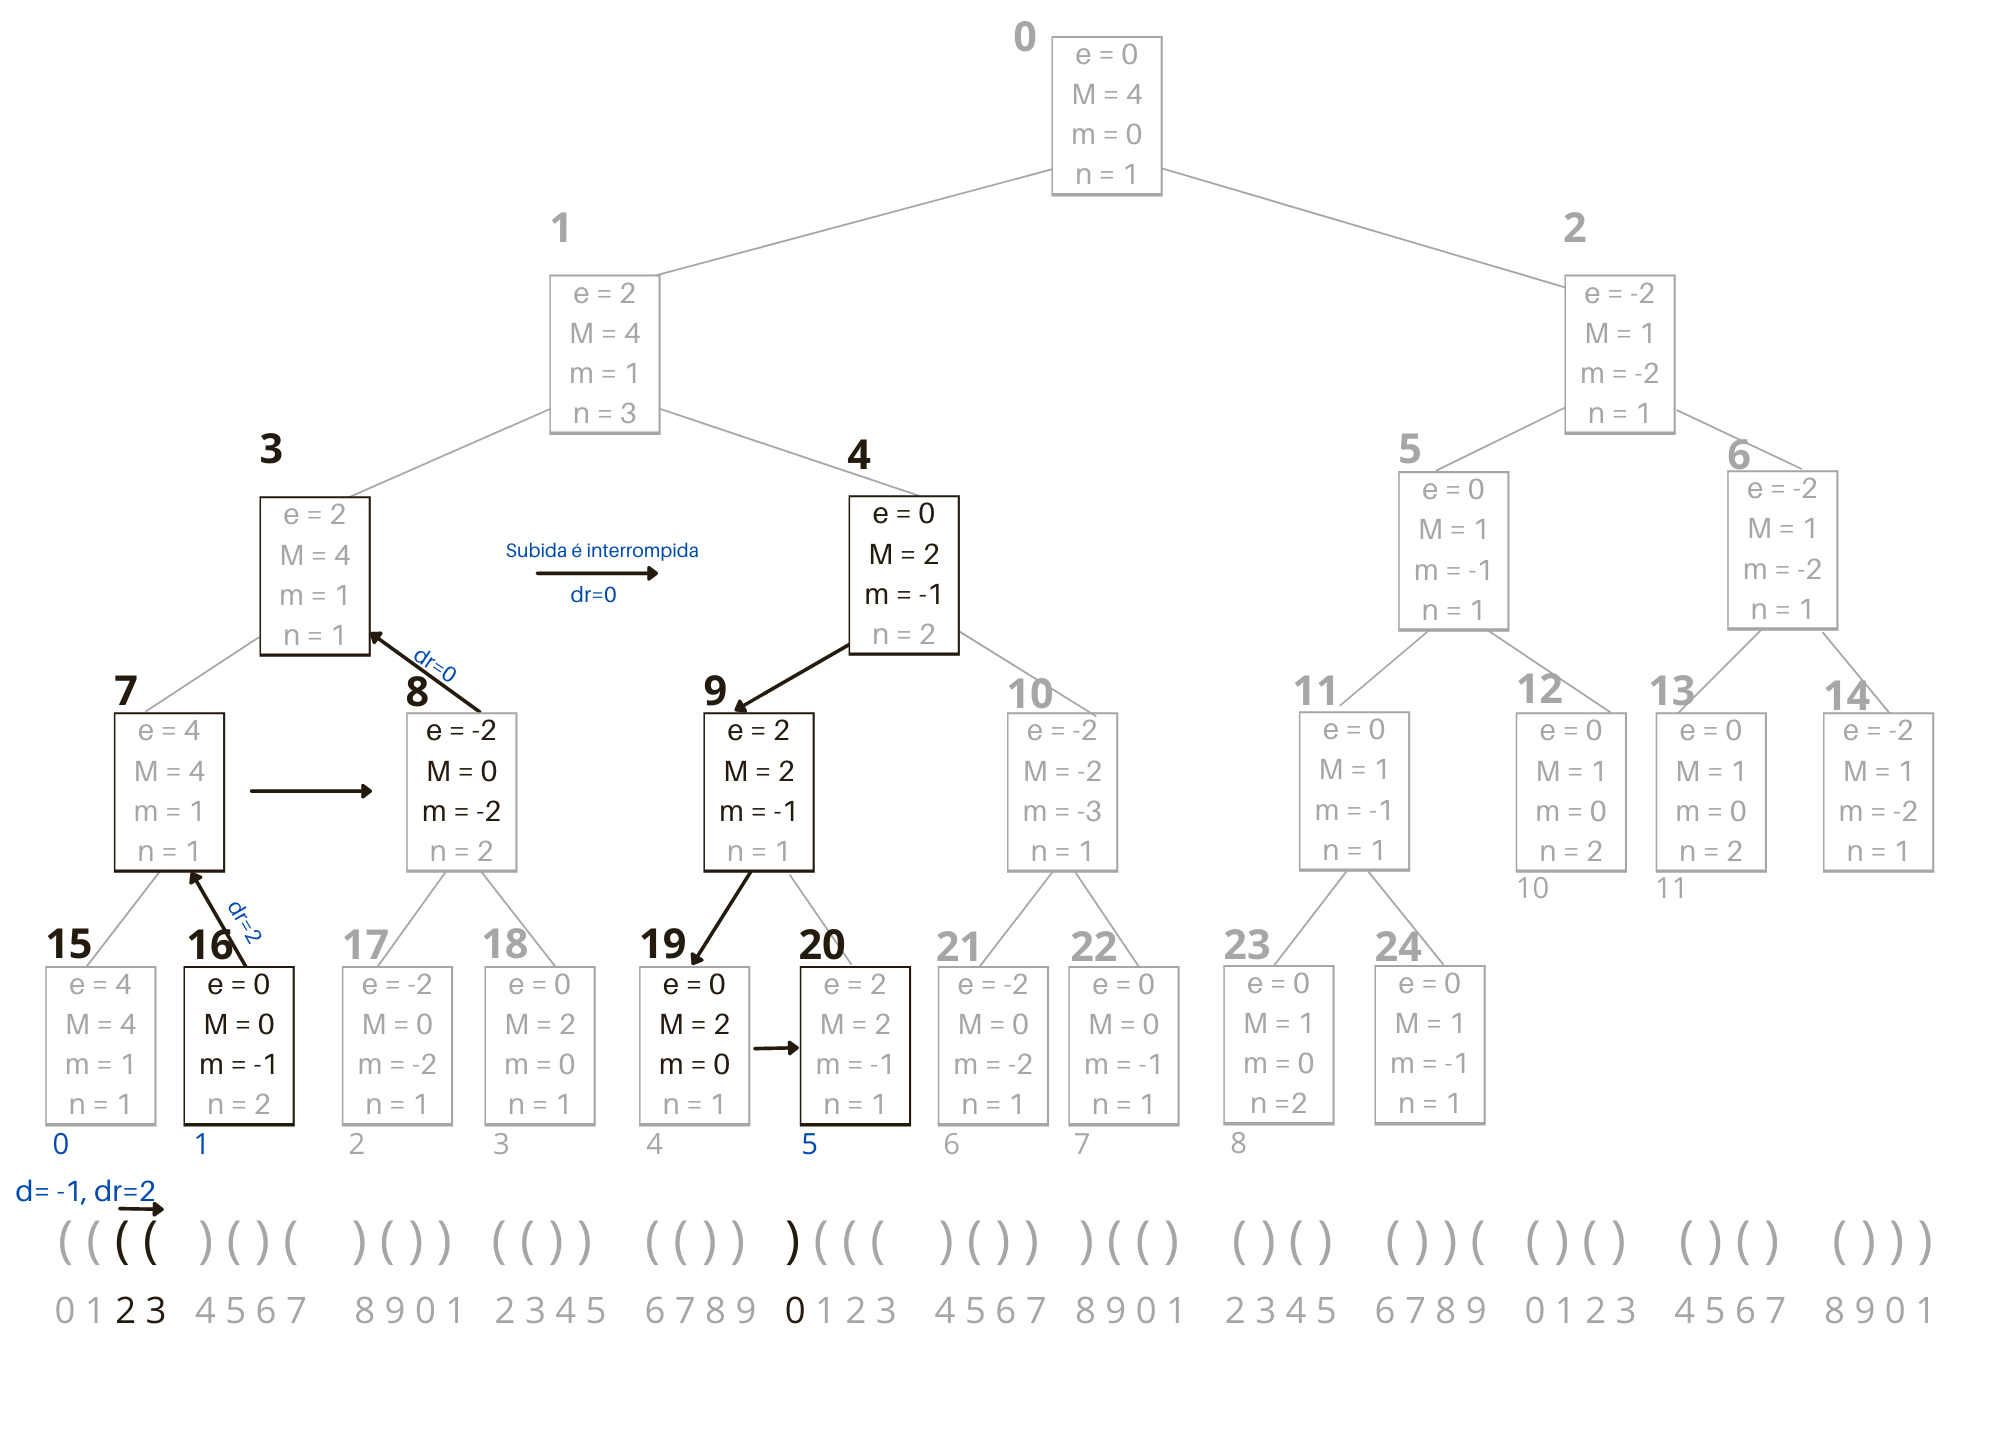
\includegraphics[scale=0.27]{images/rmm-tree-bin-fwdSearch.png}\\
         \caption{Simulação de $fwdSearch(1,-1)=20$}
     \end{figure} 
 \end{frame}

 \begin{frame}{rmM-tree: $nextSibling$}
    Problema 1: Dado um nó codificado em $i=1$, encontrar o nó codificado em $j>i$, mais à esquerda de $i$.


    Solução : 
    $$findClose(1) = fwdSearch(1,-1) = 20 $$ 



    $$nextSibling(1) = fwdSearch(1,-1) + 1 = 21 $$ 
 \end{frame}

 \begin{frame}{rmM-tree: $nextSibling$}
    Problema 1:  $nextSibling(1)$.
     \begin{figure}[h!]
         \centering
         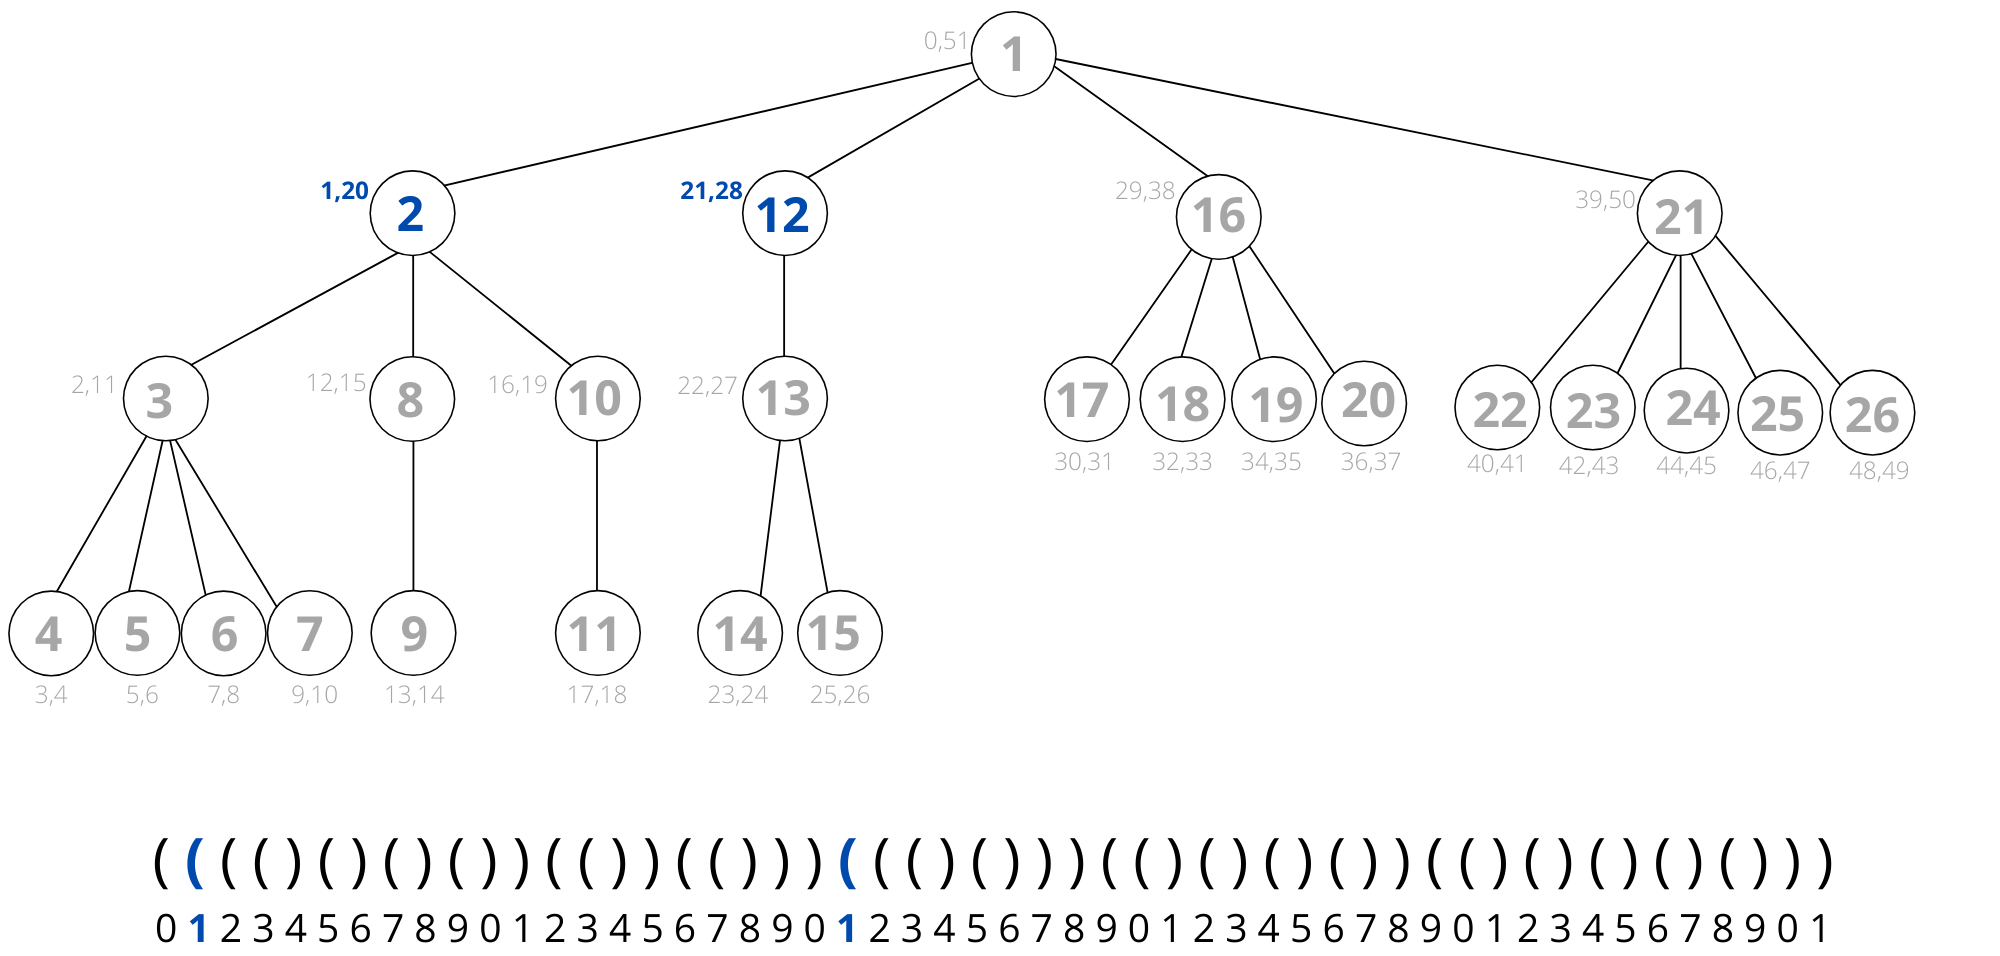
\includegraphics[scale=0.40]{images/nextSibling-res.png}\\
         \caption{Árvore de entrada}
     \end{figure} 
 \end{frame}

% \begin{frame}{rmM-tree: operações}
%     Problema 2: Verificar o ancestral comum mais baixo dos nós codificados em $i=5$ e $j=17$.
%      \begin{figure}[h!]
%          \centering
%          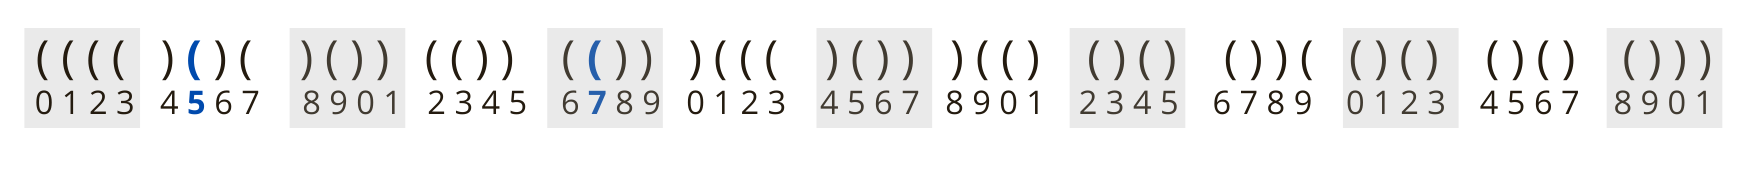
\includegraphics[scale=0.7]{images/bp-sequence.png}\\
%          \caption{Sequência de parênteses balanceados, representando uma árvore $T$}
%      \end{figure} 
 
%  \end{frame}

%  \begin{frame}{rmM-tree: $lca$}
%     Problema 2: Verificar o ancestral comum mais baixo dos nós codificados em $i=5$ e $j=17$.

%     Solução: 
%     $$lca(i,j) = 
%     \begin{cases}
%           i,  \mbox{se } isAncestor(i,j); \\
%          j, \mbox{se } isAncestor(j,i); \\
%          parent(rmq(i ,j)+1)
%     \end{cases}
%     $$ 
%  \end{frame}

%  \begin{frame}{rmM-tree: $lca$}
%     Problema 2: Verificar o ancestral comum (mais baixo) dos nós codificados em $i=5$ e $j=17$.


%     Solução:\\
%     \begin{itemize}
%         \item \textit{isAncestor(i,j)} verifica se o nó codificado em $i$ é ancestral do nó $j$;
%         \item O mesmo vale para \textit{isAncestor(j,i)};
%         \item Usar o terceiro caso.
%     \end{itemize}
%  \end{frame}


%  \begin{frame}{rmM-tree: $lca$}
%     Problema 2: Computar $lca(5,17)$.


%     Solução: $ parent(rmq(i ,j)+1)$
    

%     \begin{itemize}
%         \item $rmq(i,j) = fwdSearch(i-1, minExcess(i,j))$
   

%         \item $parent(rmq(i,j) + 1) = bwdSearch(rmq(i,j) + 1 , -2) + 1$.
%     \end{itemize}
%  \end{frame}


% \begin{frame}{rmM-tree: $lca$}
%     Problema 2: Computar $lca(5,17)$.
%      \begin{figure}[h!]
%          \centering
%          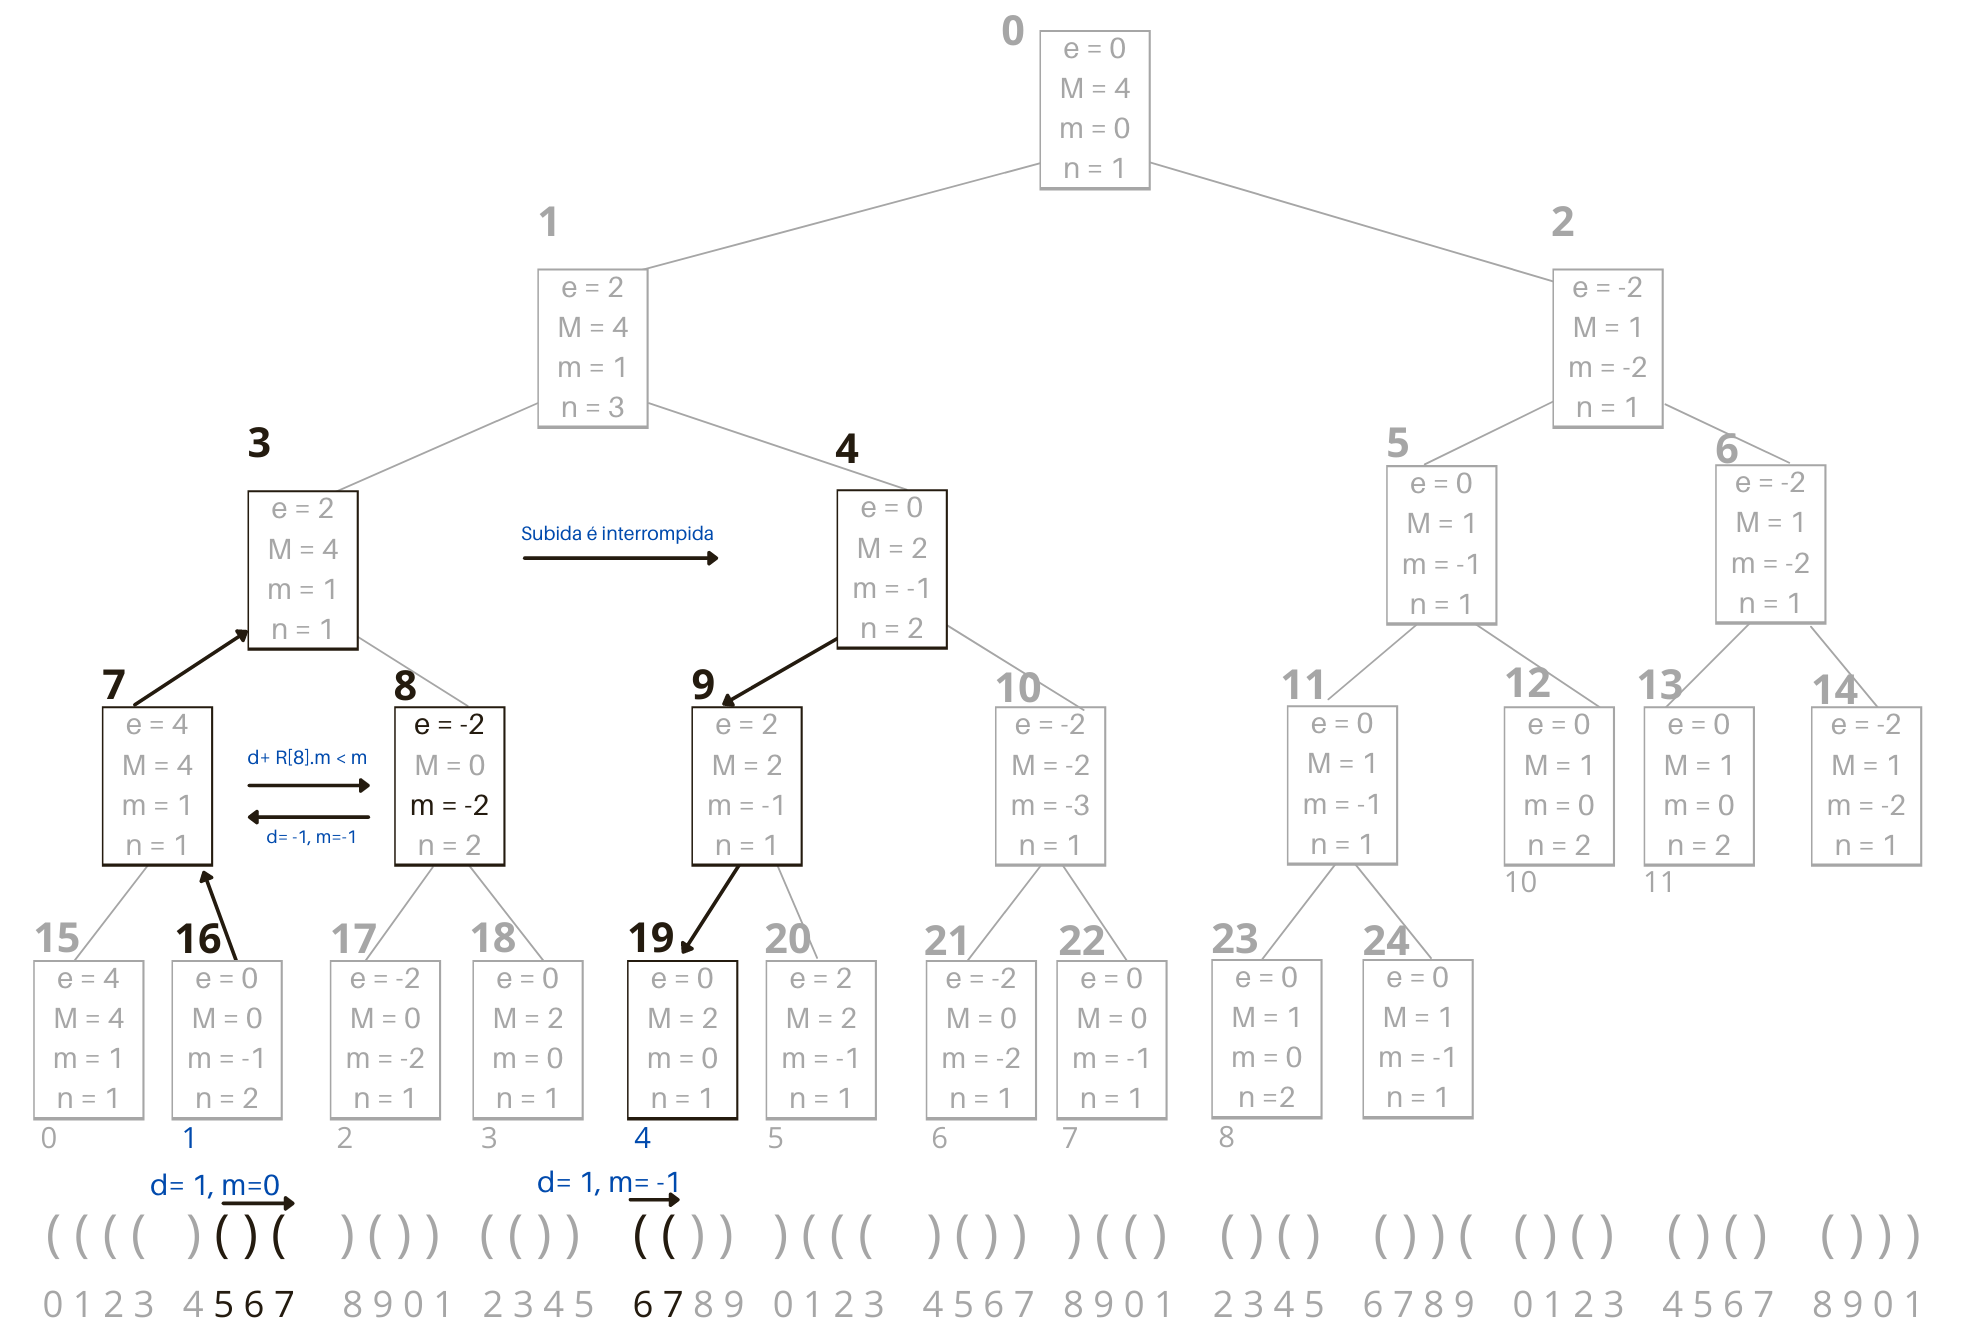
\includegraphics[scale=0.27]{images/rmm-tree-bin-minexcess.png}\\
%          \caption{Simulação de $minExcess(5,17)=-1$}
%      \end{figure} 
%  \end{frame}


% % \begin{frame}{rmM-tree: operações}
% %     Problema: Computar $lca(5,17)$.
% %      \begin{figure}[h!]
% %          \centering
% %          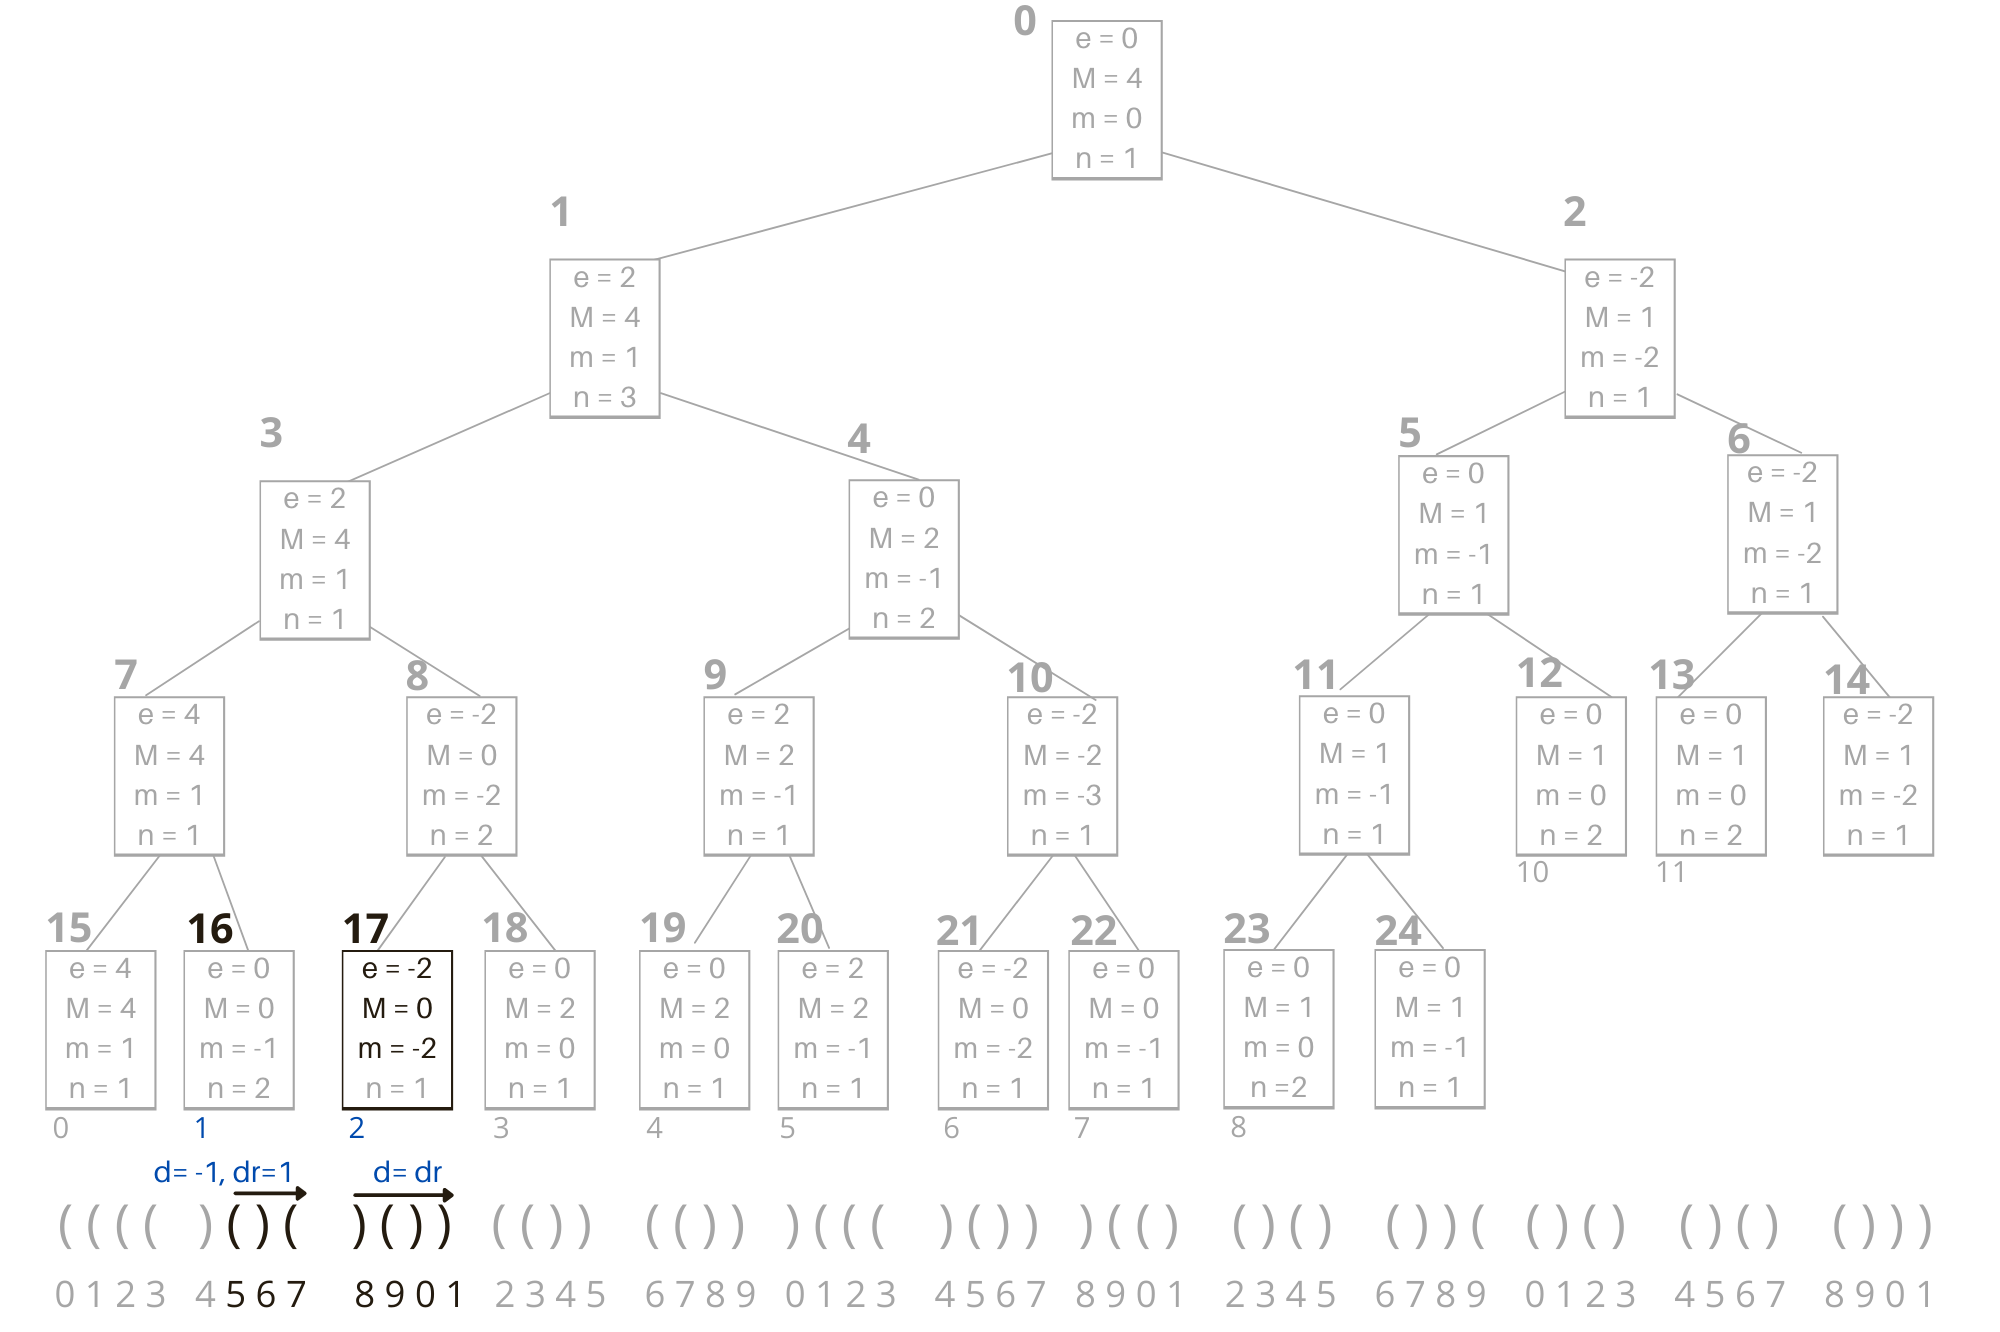
\includegraphics[scale=0.27]{images/rmm-tree-bin-fwd-lca.png}\\
% %          \caption{Simulação de $fwdSearch(4,-1)=11$}
% %      \end{figure} 
% %  \end{frame}

%  \begin{frame}{rmM-tree: $lca$}
%     Solução: Computar $lca(5,17) =  parent(rmq(5 ,17)+1)$.
%      \begin{figure}[h!]
%          \centering
%          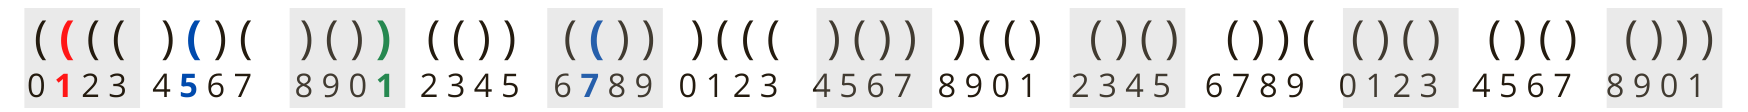
\includegraphics[scale=0.8]{images/lca-resposta.png}\\
%          \caption{Nós acessados durante a operação $lca(5,17)$}
%      \end{figure} 
%  \end{frame}

%  \begin{frame}{rmM-tree: $lca$}
%     Problema 2: Computar $lca(5,17) $.
%      \begin{figure}[h!]
%          \centering
%          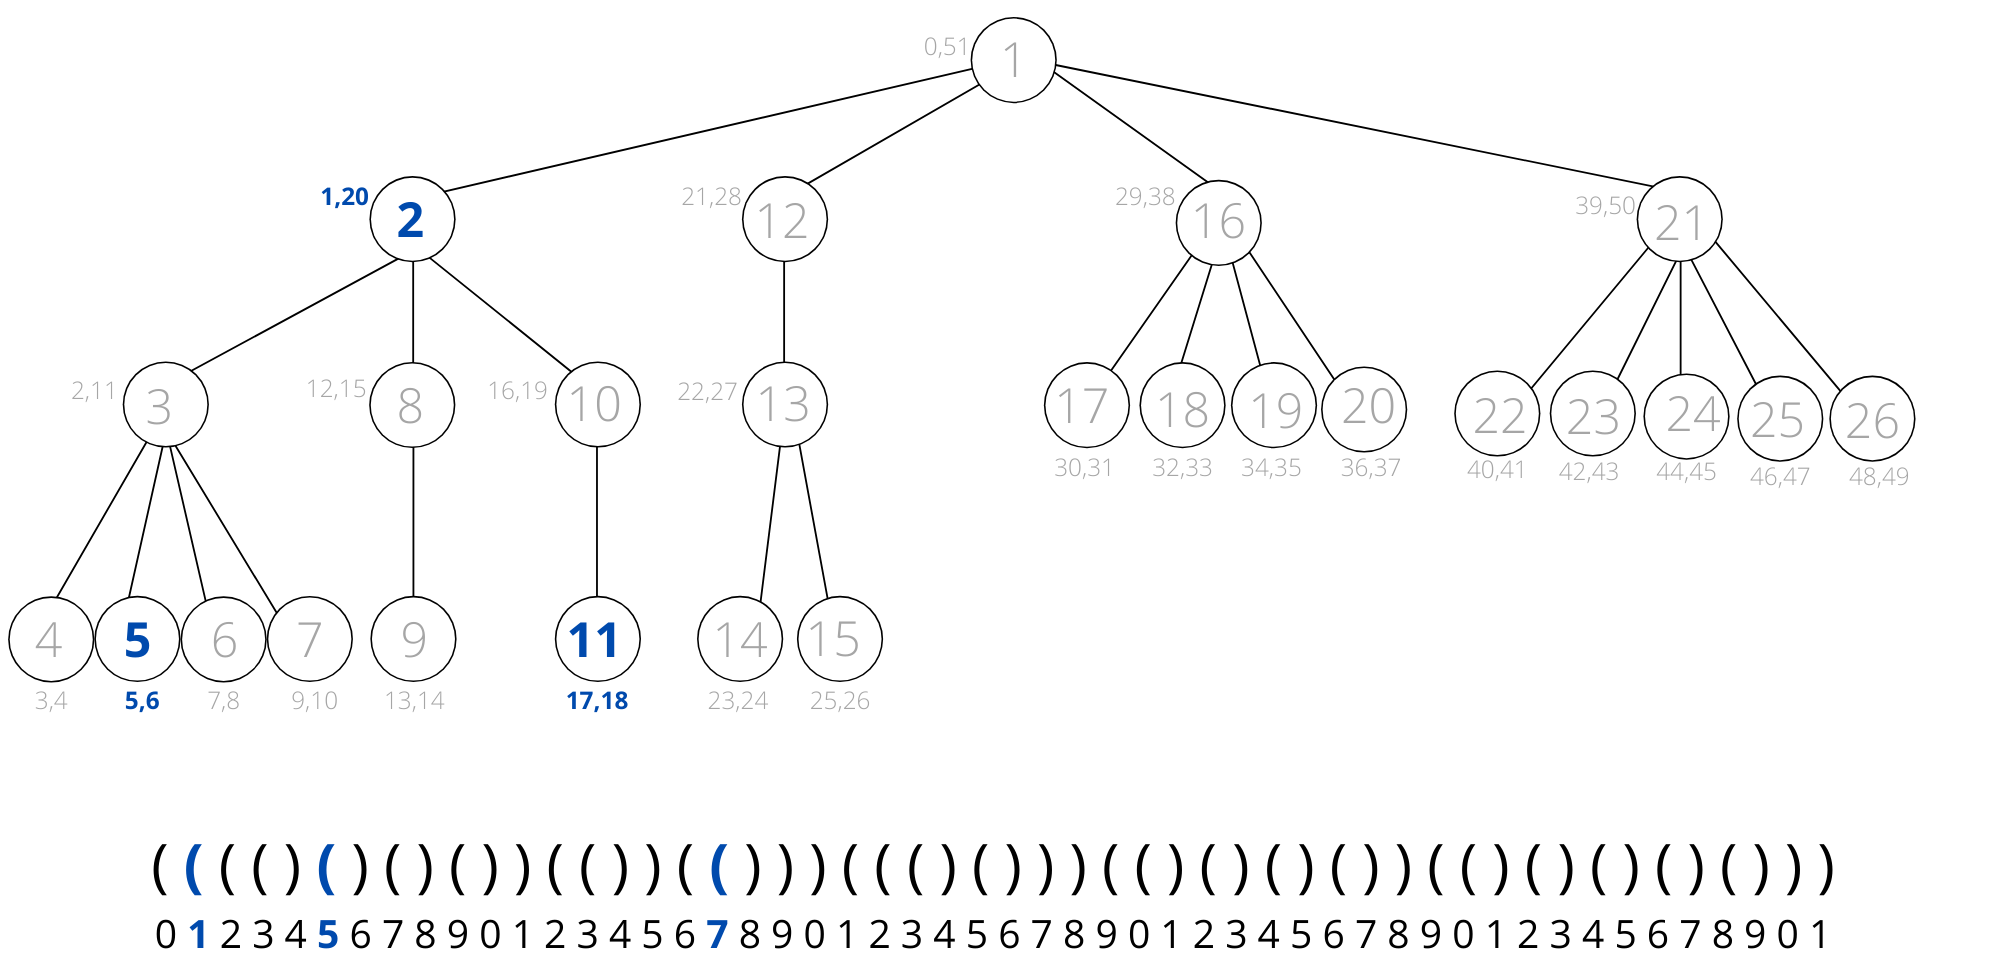
\includegraphics[scale=0.40]{images/lca-res.png}\\
%          \caption{Árvore de entrada}
%      \end{figure} 
%  \end{frame}